
\documentclass[journal,10pt,draftclsnofoot,onecolumn]{IEEEtran}

\usepackage{url}
\usepackage[tight,footnotesize]{subfigure}

% *** MISC UTILITY PACKAGES ***
%\usepackage{ifpdf}
% Heiko Oberdiek's ifpdf.sty is very useful if you need conditional
% compilation based on whether the output is pdf or dvi.
% usage:
% \ifpdf
%   % pdf code
% \else
%   % dvi code
% \fi
% The latest version of ifpdf.sty can be obtained from:
% http://www.ctan.org/tex-archive/macros/latex/contrib/oberdiek/
% Also, note that IEEEtran.cls V1.7 and later provides a builtin
% \ifCLASSINFOpdf conditional that works the same way.
% When switching from latex to pdflatex and vice-versa, the compiler may
% have to be run twice to clear warning/error messages.

% *** CITATION PACKAGES ***
%
%\usepackage{cite}
% cite.sty was written by Donald Arseneau
% V1.6 and later of IEEEtran pre-defines the format of the cite.sty package
% \cite{} output to follow that of IEEE. Loading the cite package will
% result in citation numbers being automatically sorted and properly
% "compressed/ranged". e.g., [1], [9], [2], [7], [5], [6] without using
% cite.sty will become [1], [2], [5]--[7], [9] using cite.sty. cite.sty's
% \cite will automatically add leading space, if needed. Use cite.sty's
% noadjust option (cite.sty V3.8 and later) if you want to turn this off
% such as if a citation ever needs to be enclosed in parenthesis.
% cite.sty is already installed on most LaTeX systems. Be sure and use
% version 5.0 (2009-03-20) and later if using hyperref.sty.
% The latest version can be obtained at:
% http://www.ctan.org/tex-archive/macros/latex/contrib/cite/
% The documentation is contained in the cite.sty file itself.

% *** GRAPHICS RELATED PACKAGES ***
%
\ifCLASSINFOpdf
  \usepackage[pdftex]{graphicx}
  % declare the path(s) where your graphic files are
  % \graphicspath{{../pdf/}{../jpeg/}}
  % and their extensions so you won't have to specify these with
  % every instance of \includegraphics
  \DeclareGraphicsExtensions{.pdf,.jpeg,.png}
\else
  % or other class option (dvipsone, dvipdf, if not using dvips). graphicx
  % will default to the driver specified in the system graphics.cfg if no
  % driver is specified.
  % \usepackage[dvips]{graphicx}
  % declare the path(s) where your graphic files are
  % \graphicspath{{../eps/}}
  % and their extensions so you won't have to specify these with
  % every instance of \includegraphics
  % \DeclareGraphicsExtensions{.eps}
\fi


% correct bad hyphenation here
\hyphenation{op-tical net-works semi-conduc-tor}


\begin{document}

\title{Tracking the Diffusion of Named Entities}


\author{TBD}% <-this % stops a space

% The paper headers
\markboth{Computational Intelligence Magazine}
{Shell \MakeLowercase{\textit{et al.}}: Tracking the Diffusion of Named Entities}

% make the title area
\maketitle

% As a general rule, do not put math, special symbols or citations
% in the abstract or keywords.
\begin{abstract}
To do
\end{abstract}

% Note that keywords are not normally used for peerreview papers.
\begin{IEEEkeywords}
To do
\end{IEEEkeywords}

\IEEEpeerreviewmaketitle



\section{Introduction}

The aim of this paper is to understand how named entities \emph{emerge} and \emph{spread} through social media based discourse.
We are interested in exploring the following research questions:
\begin{enumerate}
	\item \textbf{RQ1:} How can we accurately detect named entities in social media based discourse, given its myriad formats, often informal vernacular, and inherent noise (e.g. misspellings, abbreviations, etc.)?
	\item \textbf{RQ2:} Under what conditions do entity mentions diffuse through discourse? And when are people \emph{most likely} to be influenced into then discussing entities?
	\item \textbf{RQ3:} How can we predict the discussion of certain named entities and who will begin talking about them?	
\end{enumerate}


\section{Datasets}
For this research we will use the following datasets:

\begin{enumerate}
	\item Reddit data -- download and access all of the data from the full dump.\footnote{\url{https://archive.org/details/2015_reddit_comments_corpus}}
	\item CoNLL 2003 data -- a corpus of newswire texts, annotated for named entity chunks and types.
	This describes where entity mentions are in the text, including locations, organisations, and person mentions.
	\item Twitter data; unannotated -- we have a large corpus of English tweets that we can use here.
	\item Twitter data; annotated -- there are two datasets annotated with named entities. These are from Ritter's 2011 EMNLP paper, and the W-NUT 2015 shared task.
\end{enumerate}


\section{Research Stages}

\subsection{Stage 0: Data Preparation and NER}
-To do:\\
--Annotate corpora with detected entities using basic typing of: person, location, organisation\\
--Run NER software over dataset and validate accuracy of this (using basic measures)\\
--Run NER over entire dataset to extract entities

\subsection{Stage 1: Exploratory Analysis}
-To do:\\
--Plot relative frequency distribution as a function of time for named entities, and characterise the \emph{shape} of the entities\\
--Apply lifecycle model to profile users' NER citations over time and investigate how users' profiles are influenced by global, community, and prior behaviour dynamics

\subsection{Stage 2: Diffusion Analysis}
-To do:\\
--Model the spread of named entities through user profiles (could use multivariate diffusion models here)

\subsection{Stage 3: Forecasting}
-To do:\\
--Implement models to forecast if a user will mention an entity and who that will be (hard!)


%-----------------------------------------------------

\section{Related work}

twitter info propagation

reddit compared to other OSNs: "Lifespan and propagation of information in On-line Social Networks: A case study based on Reddit"  http://www.sciencedirect.com/science/article/pii/S1084804515001307

network structure of reddit: "Navigating the massive world of reddit: using backbone networks to map user interests in social media" https://peerj.com/articles/cs-4/

twitter nlp


\section{Data preparation and NER}

To conduct our study, we need to convert 140GB of compressed Reddit posts into a set of interlinked and time-ordered conversations and the entities mentioned in each of them.
This provides a number of sub-challenges: sampling of the Reddit data, creating a linked series of conversations, and picking out entity mentions in this text type.
Reddit data is largely unexplored in the NLP community, despite the large volume of it and the especially rich metadata.
This poses additional challenges: certainly, given the lack of work on Reddit text, there are no annotated datasets available yet, so supervised in-domain work is not directly possible yet.
Additionally, the datasets are large, which makes it important to choose a good subset of data on which to do prototyping and development, in order to keep research cycles short.
The result that we come to at the end of this stage is a rich dataset for tracking entity and concept diffusion within and across communities.

\begin{figure}
\centering
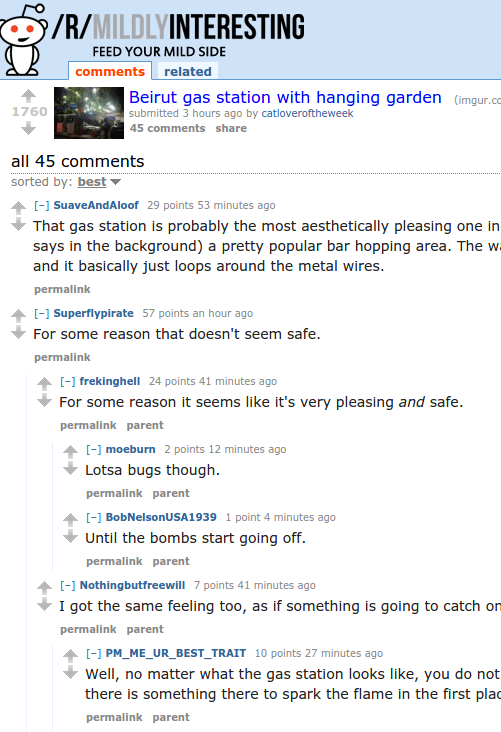
\includegraphics[width=0.4\columnwidth]{reddit-example.png}
\label{fig:reddit-example}
\caption{Example discussion around a Reddit post.}
\end{figure}

The Reddit dataset~\cite{reddit-data} is comprised of a sequence of comments, with one JSON record for each one.
These are ordered temporally.
Reddit itself is roughly similar to a forum, where top-level divisions are made by topic.
Within each topic, or {\em subreddit}, there are posts, which begin with either a short piece of text or a link to an external resource -- typically an image, video, or interesting article.
Users then may publish comments for each post, and reply to each others' comments.
This leads to a threaded discussion, centred on a particular topic, with a hierarchical comment structure (see Figure~\ref{fig:reddit-example}).


\subsection{Subreddit extraction}

- subreddit extraction

top lists

describe top lists site

pick 100

extract these over whole sample

figures for raw dataset (\# per year; total volume over time; volume-rank graph of subreddits; possible ref to appx)

\subsection{NER for Reddit}

-- where is NER first mentioned and defined?

We model micro-topics in conversation as entity mentions.
This allows tracking of topics at maximally fine granularity, looking at each user's interests at a low level, as opposed to monitoring broader topics such as ``consumer electronics", ``politics" and so on.
In fact, these broader topics are already explicitly annotated by means of the subreddit topics.

Entity mentions are extracted through named entity recognition.
Generally, this task aims to detect the boundaries of certain kinds of entities within a certain piece of text.
In this instance, we tokenise text, splitting it into sentences using the Punkt tokeniser~\cite{kiss2006unsupervised}, and subsequently word-sized chunks, using the {\tt twokenize} tool with some adaptations~\cite{o2010tweetmotif}.
This tool performs Penn Treebank-style tokenisation, a common standard, with some specific adaptations to enable it to handle the noise present in user-generated text.
After this, we take a structured prediction approach to deciding which tokens in each sentence are part of an entity, and possibly the type of the entity.
Finally, we concatenate entity tokens, and use these to build a list of entity mentions in any given input text.
For example, given the input comment from the source JSON:

\begin{quote}
``body": ``There are still some really good fighters on this card. Conor McGregor is on the card and so is Gunnar Nelson."
\end{quote}

The following output entities should be collected:

\begin{quote}
``entity\_texts": [``Conor McGregor", ``Gunnar Nelson"]
\end{quote}

Typically, many NER systems take a supervised approach; that is, they use data labelled by humans as training data, from which features are extracted to form training instances for a machine learning algorithm.
However, NLP systems can be hard to transfer between text types; for example, NER systems for newswire might reach about 89\% F1 on news articles, but only around 40\% on tweets (a form of user-generated content), as found in~\cite{derczynski2015analysis}.
One approach to overcoming this performance drop when changing text type is to train over a blend of text types.
For example, Ritter~\cite{ritter2011named} used both IRC\footnote{Internet Relay Chat -- informal internet conversation text} and newswire data when developing a part-of-speech tagger for tweets, as well as an unsupervised language model from the target text type.
This led to strong performance improvements.
We follow a similar approach, using a blend of NE-annotated corpora from both newswire and tweets.
The newswire data is drawn from the CoNLL-2003 evaluation task set~\cite{tjong2003introduction}; the twitter data is from Ritter's early experiments and also the W-NUT 2015 shared task~\cite{ritter2011named,baldwin2015shared}.

We start using structured predicting in the form of a CRF to label whole sentences at a time.
For features, we use a fairly classical set, and add some unsupervised word representations to this.
Our base features are:

\begin{itemize}
\item 
\end{itemize}

In addition, we induce Brown clusters~\cite{brown1992class} and use these as word representations~\cite{turian2009preliminary}.
Brown clustering is a form of hierarchical agglomerative hard clustering, using average mutual information as its objective function.
It takes as input a corpus, in the form of a sequence of words, and in its generalised form~\cite{derczynski2016generalised}, a single hyperparameter: the size of its active set $a$.
The result is a sequence of binary merges, describing the set membership of each word type in the corpus as the merges progress.
For each single word type, therefore, the path to a destination cluster can be described as a bitstring, which details the sequence of binary merges taken.
The zero-length bitstring describes the situation at the top of the hierarchy, where there is one class.

These bitstrings are typically converted to features by shearing.
This involves only examining the first $n$ bits of a bitstring.
However, shearing does not maximise the information preserved in the representation -- sub-clusterings at many levels are lost.
We therefore experiment with a new method of feature extraction form Brown clusters, which we call {\em provenance-based} feature extraction.
We take the cluster identifier at every level, tracing the provenance of a terminal word cluster all the way to the root cluster (which contains all word types).
This preserves the entire set membership of any given term, throughout the induced hierarchical clustering.
As an example, if the term \emph{fishing} has bitstring $1100101$, the following text features are generated: $1$, $11$, $110$, $1100$, $11001$, $110010$, $1100101$.
For contrast, if the typical bit depths of 4, 6, 10 and 20~\cite{ratinov2009design} were chosen, only the following features would be generated: $1100$, $110010$, $1100101$.
As a result of taking all directly-relevant features in the merge list, the lossy nature of shearing-based feature extraction from Brown clusters is avoided.

Feature extraction, training, classification and JSON annotation are all performed using an entity recognition toolkit (https://github.com/leondz/entity\_recognition~\cite{derczynski2015usfd}), with custom extractors.


\subsection{Tuning entity recognition}

Entity recognition needs to be tuned to fit Reddit data well.
There are a number of parameters in our training data balance, feature extraction, and objective function that all reflect the nature of the data and the task at hand.
We present our method for estimating of these factors, and intrinsic NER evaluation.

In terms of evaluation, we prefer recall over precision.
Over the large dataset, spurious entities are likely to be those that are not seen very often or have an unusual pattern.
This suggests that there will be great variation in their surface forms, leaving them in the long tail of discovered entities.
As the majority of our work looks at the more frequent patterns, these are less likely to have an impact.
Conversely, recall reveals how well the extraction is performing, and it important to track a range of entities.
In addition, recall has always been more challenging to achieve in social media texts than recall~\cite{ritter2011named,derczynski2015analysis}.

To capture this balance, we take F-scores with $\beta=2$.
Given precision $P$ and recall $R$, typically an F-score is drawn from $F_\beta$ with $\beta=1$.

\begin{equation}
F_\beta = (1+\beta^2)\frac{PR}{(\beta^2 P) + R} 
\end{equation}

When $\beta=1$, precision and recall are balanced in a harmonic mean, e.g. F1-score.
That is, false positives and false negatives impact results equally.
To score away from false positives, i.e. wrong cues, we set $\beta=2$.

Our approach here is to tune an entity recogniser with reference to a dataset that matches the target text type.
We draw this development set from Reddit posts, using comments encountered during our work that appear to have missing or spurious annotations.
These are then isolated, tokenised, and manually annotated.
Our annotation format follows~\cite{ritter2011named} in using the Freebase top-level entity type inventory, but only uses the chunking information, as nothing further than this is needed: only the surface forms of entities.
In total, we identified and annotated 3\,708 tokens of Reddit data, including 149 entity chunks.
This comprised our development set, which was used to tune a variety of parameters in our approach.

Firstly, we tuned our word representations.
Specifically, we needed to estimate the number of Brown clusters $C$ to use in feature extraction.
We also then used this to determine what blend of social, Reddit or news data gave best results in unsupervised feature generation and extraction.
To tune the value for $C$, we examined a similar scenario with similar dataset sizes, and estimated an optimum.
We noted that in prior work~\cite{derczynski2015tune}, entity recognition performance with decomposed class prefixes -- similar to the provenance-based features we propose here -- peak at around $C=2500$ for corpora of 16k tokens, $C=5000$ for corpora of 32k tokens, and at higher values for larger datasets.
As General Brown clustering is dependent on the number of types and the size of the active set $a$, and results are unreliable with $a>C$, we set $C = a = 4000$.
We then experiment with combinations of newswire, Twitter and Reddit data.
Brown clusters are extracted using the generalised-brown package~\cite{sean_chester_2015_33758}.
Results are given in Table~\ref{tab:brown-tuning}.

-- results of brown cluster tuning


In addition, we draw supervised data for multiple datasets in order to approximate the Reddit text type.
We take data from Reddit, taking the union of corpora used in previous work that follow the Freebase ten-class entity scheme~\cite{ritter2011named,baldwin2015shared}.
This scheme gives broader coverage than e.g. the three-class ACE named entity scheme.
For newswire, we use the Reuters RCV1 corpus annotations that were part of the CoNLL-2003 shared task~\cite{tjong2003introduction}.
Classes are removed before training, making this just a chunking task.
We compare against Stanford NER~\cite{finkel2005incorporating} as a baseline.
Results for different balances of training data are given in Table~\ref{tab:supervision-balance}


-- analysis of cross-genre ne chunking performance


Note that while some figures seem low when compared to typical newswire level performance, the toolkit used is high-ranking, state-of-the-art research software, coming third in the 2015 W-NUT challenge for entity chunking over tweets.
The task is simply difficult; Twitter NER recall has always been low.
In addition, it is a generally consistent finding that generalising NER systems beyond newswire is not yet well understood; systems that perform very well on this text type (e.g. F1 of 0.89 from Stanford NER~\cite{derczynski2013microblog}) can often score very poorly on social media content (F1 of 0.41).
This may be due to overfitting of tools to newswire over time, due to community challenges, dataset in just one type, extra custom rules adapting to formal news text, or other things -- but this is beyond the scope of this paper.
We do note that our approach uses largely unsupervised feature extraction and performs better than on other social media corpora, also beating the Stanford NER system, in this first attempt at named entity chunking for Reddit.


\clearpage
\section{Entity Diffusion}

\subsection{Entity Mention Cascades}
-Describe the entity cascade graphs and what these entail
-Explain how these were derived using graph isomorphism and then the rank induced

\begin{figure}[ht!]
  \begin{center}
  \subfigure[Cascade Shapes]{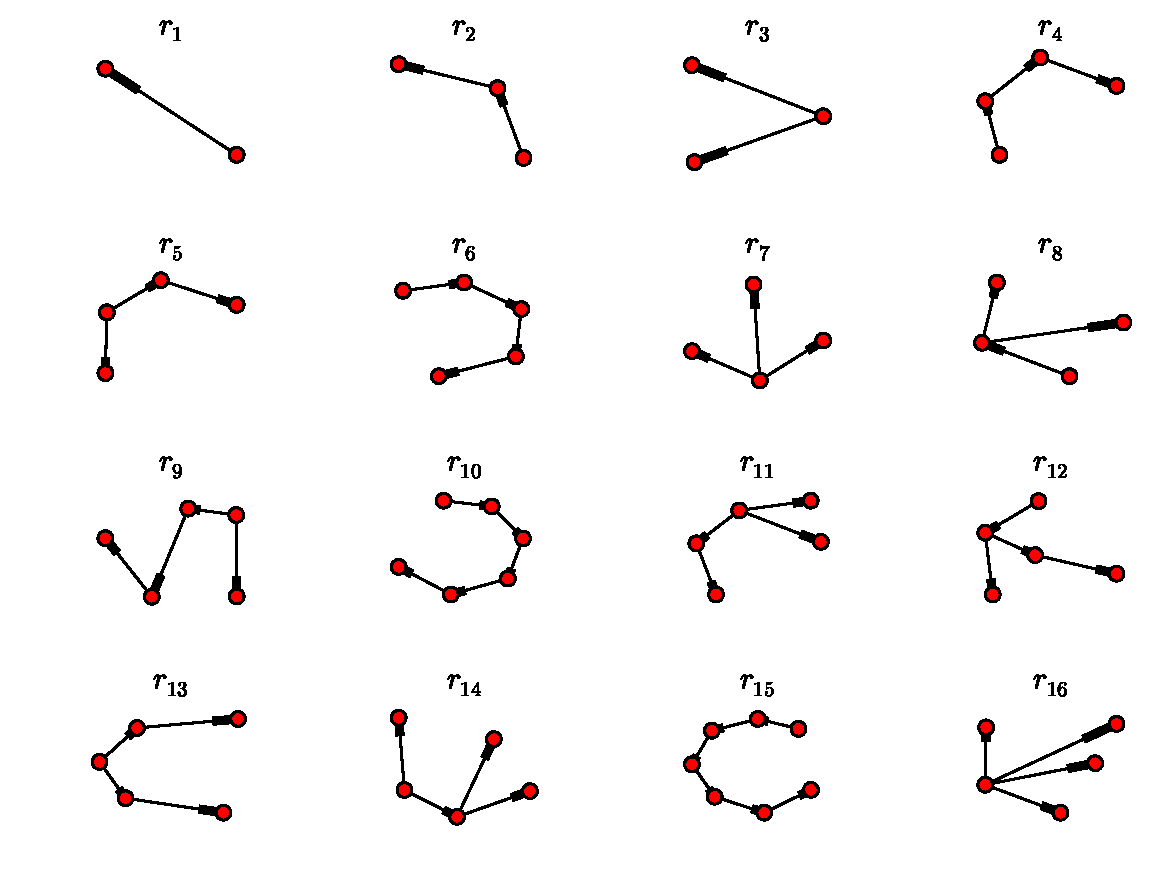
\includegraphics[width=0.49\columnwidth]{plots/cascade_shapes.pdf}\label{fig:cascade_shapes}}   
  \subfigure[Shape Rank Distribution]{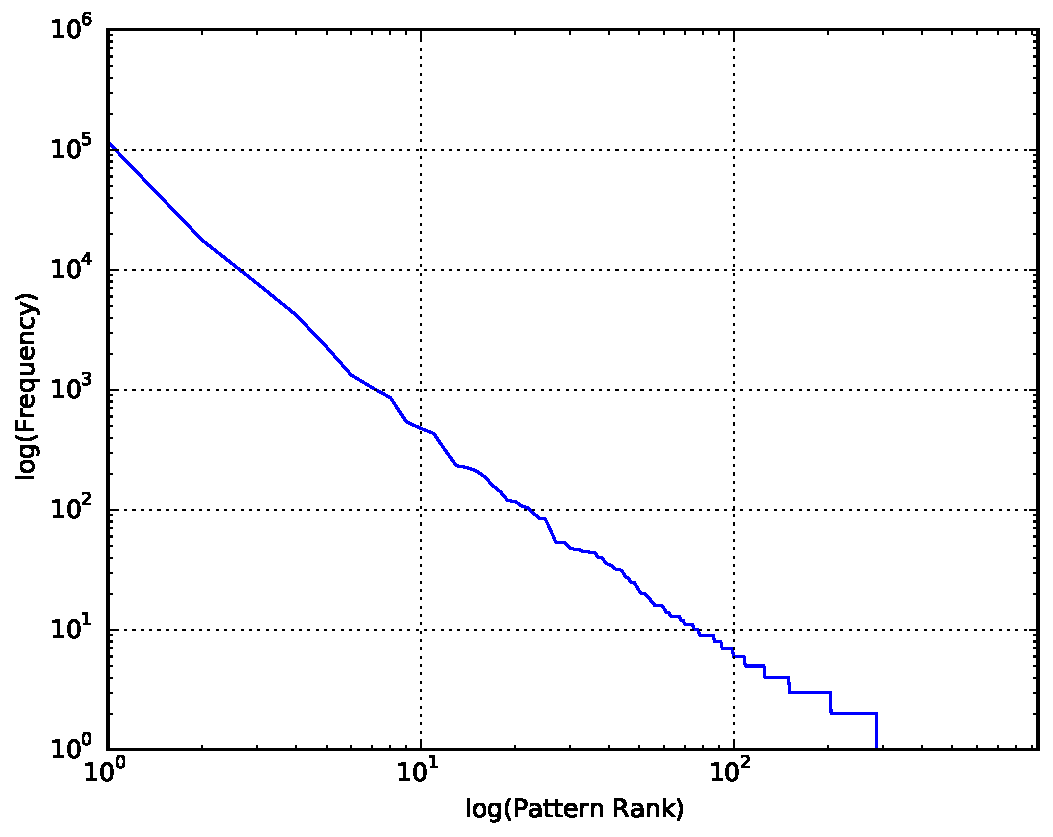
\includegraphics[width=0.49\columnwidth]{plots/cascade_rank_dist.pdf}\label{fig:rank_dist}}
  \end{center}    
  \caption{To do}
  \label{fig:entity_cascades}
\end{figure}


\subsection{Entity Adoption Post-${k-1}^{th}$ Exposure}
-Potential for adoption at the point of one exposure
-Per entity-exposure dynamics - add plots of random selection of entities

\begin{figure}[ht!]
  \begin{center}
  \subfigure[Exposure-Adoption Global Distribution]{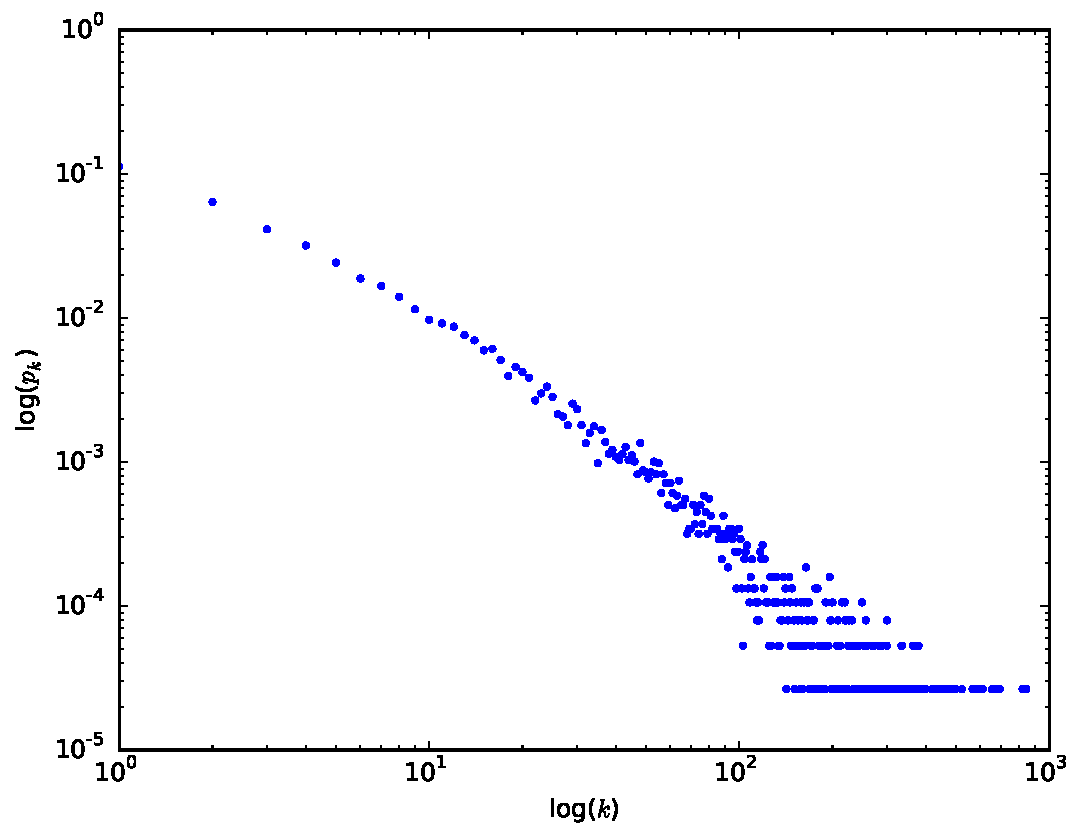
\includegraphics[width=0.49\columnwidth]{plots/exposure_count_dist_full_log.pdf}\label{fig:global_exposure_dist}}   
  \subfigure[Random Entity Exposure-Adoption Distributions]{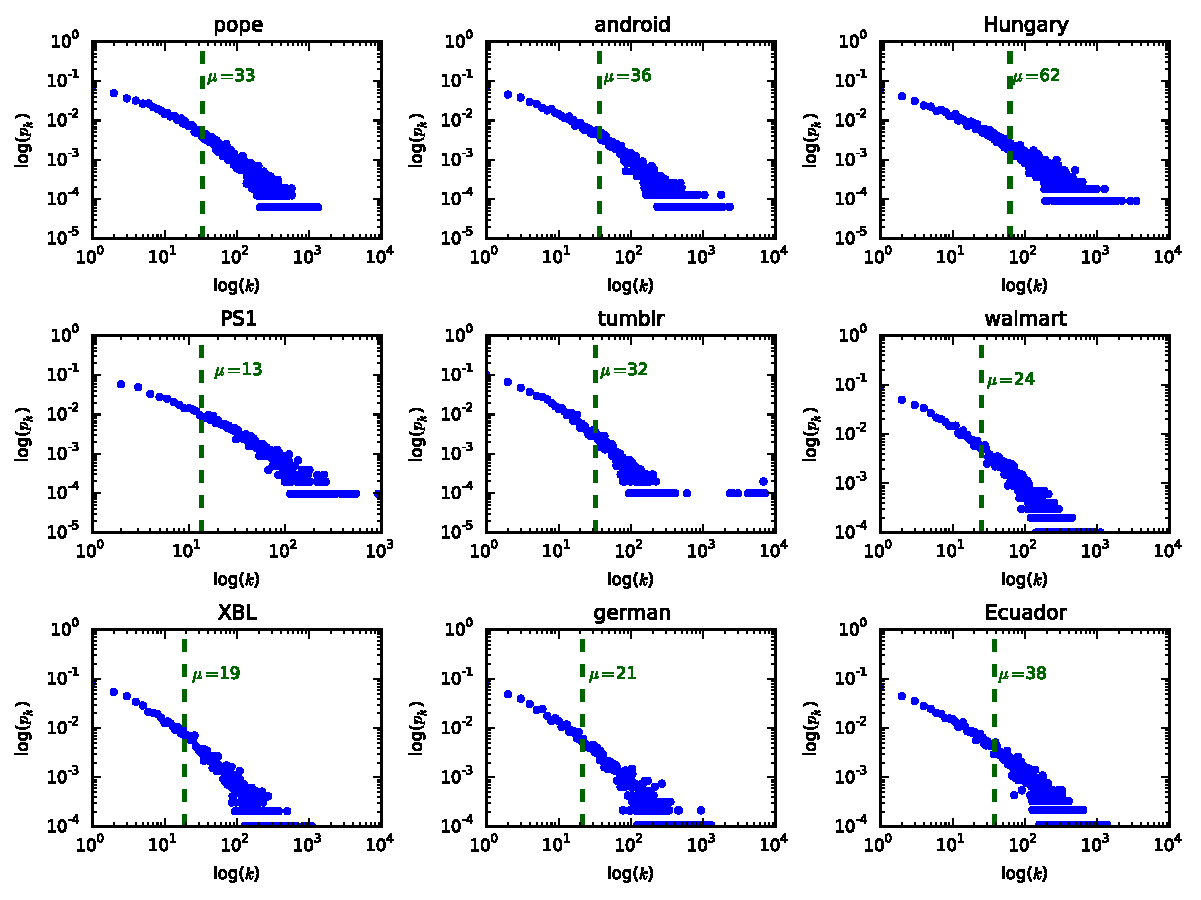
\includegraphics[width=0.49\columnwidth]{plots/per_entity_exposure_count_dist_full_log.pdf}\label{fig:entity_exposure_dists}}
  \end{center}    
  \caption{To do}
  \label{fig:exposure_dists}
\end{figure}



\subsection{Global Threshold Diffusion Model}
-Explain the implementation of WSDM2010 work and adaptation for non-sequential dataset scans - necessary due to memory load being infeasible

\subsubsection{Distribution of $\tau_{v,u}$}
-Present the distribution of $\tau_{v,u}$ and what this implies for the model

\begin{figure}[ht!]
  \begin{center}
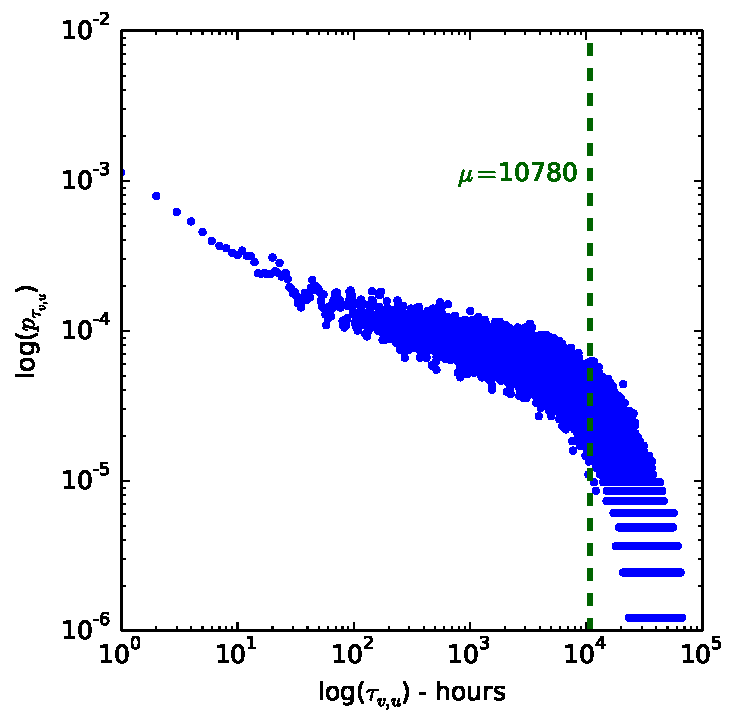
\includegraphics[width=0.49\columnwidth]{plots/taus_dist_full_log.pdf}
  \end{center}    
  \caption{To do}
  \label{fig:taus_dist}
\end{figure}


\subsection{Experiments}
-Explain the evaluation process and the computation of the ROC values - per entity
-Plot variance in the ROC values achieved



% if have a single appendix:
%\appendix[Proof of the Zonklar Equations]
% or
%\appendix  % for no appendix heading
% do not use \section anymore after \appendix, only \section*
% is possibly needed

% use appendices with more than one appendix
% then use \section to start each appendix
% you must declare a \section before using any
% \subsection or using \label (\appendices by itself
% starts a section numbered zero.)
%


%\appendices
%\section{Proof of the First Zonklar Equation}
%Appendix one text goes here.
%
%% you can choose not to have a title for an appendix
%% if you want by leaving the argument blank
%\section{}
%Appendix two text goes here.
%
%
%% use section* for acknowledgment
%\section*{Acknowledgment}
%
%
%The authors would like to thank...
%
%
%% Can use something like this to put references on a page
%% by themselves when using endfloat and the captionsoff option.
%\ifCLASSOPTIONcaptionsoff
%  \newpage
%\fi



% trigger a \newpage just before the given reference
% number - used to balance the columns on the last page
% adjust value as needed - may need to be readjusted if
% the document is modified later
%\IEEEtriggeratref{8}
% The "triggered" command can be changed if desired:
%\IEEEtriggercmd{\enlargethispage{-5in}}

% references section

% can use a bibliography generated by BibTeX as a .bbl file
% BibTeX documentation can be easily obtained at:
% http://www.ctan.org/tex-archive/biblio/bibtex/contrib/doc/
% The IEEEtran BibTeX style support page is at:
% http://www.michaelshell.org/tex/ieeetran/bibtex/
\bibliographystyle{IEEEtran}
% argument is your BibTeX string definitions and bibliography database(s)
%\bibliography{IEEEabrv,NER-Diffusion}
\bibliography{NER-Diffusion}
%
% <OR> manually copy in the resultant .bbl file
% set second argument of \begin to the number of references
% (used to reserve space for the reference number labels box)
%\begin{thebibliography}{1}
%
%\bibitem{IEEEhowto:kopka}
%H.~Kopka and P.~W. Daly, \emph{A Guide to \LaTeX}, 3rd~ed.\hskip 1em plus
%  0.5em minus 0.4em\relax Harlow, England: Addison-Wesley, 1999.
%
%\end{thebibliography}
%
%% biography section
%% 
%% If you have an EPS/PDF photo (graphicx package needed) extra braces are
%% needed around the contents of the optional argument to biography to prevent
%% the LaTeX parser from getting confused when it sees the complicated
%% \includegraphics command within an optional argument. (You could create
%% your own custom macro containing the \includegraphics command to make things
%% simpler here.)
%%\begin{IEEEbiography}[{\includegraphics[width=1in,height=1.25in,clip,keepaspectratio]{mshell}}]{Michael Shell}
%% or if you just want to reserve a space for a photo:
%
%\begin{IEEEbiography}{Michael Shell}
%Biography text here.
%\end{IEEEbiography}
%
%% if you will not have a photo at all:
%\begin{IEEEbiographynophoto}{John Doe}
%Biography text here.
%\end{IEEEbiographynophoto}
%
%% insert where needed to balance the two columns on the last page with
%% biographies
%%\newpage
%
%\begin{IEEEbiographynophoto}{Jane Doe}
%Biography text here.
%\end{IEEEbiographynophoto}

% You can push biographies down or up by placing
% a \vfill before or after them. The appropriate
% use of \vfill depends on what kind of text is
% on the last page and whether or not the columns
% are being equalized.

%\vfill

% Can be used to pull up biographies so that the bottom of the last one
% is flush with the other column.
%\enlargethispage{-5in}



% that's all folks
\end{document}


